% Figure: environment-to-import migration map (story 1).
% Build: pdflatex environ_migration.tex  (run inside figures/)
\documentclass[tikz,border=6pt]{standalone}
\usetikzlibrary{positioning,arrows.meta,fit,backgrounds}
\begin{document}
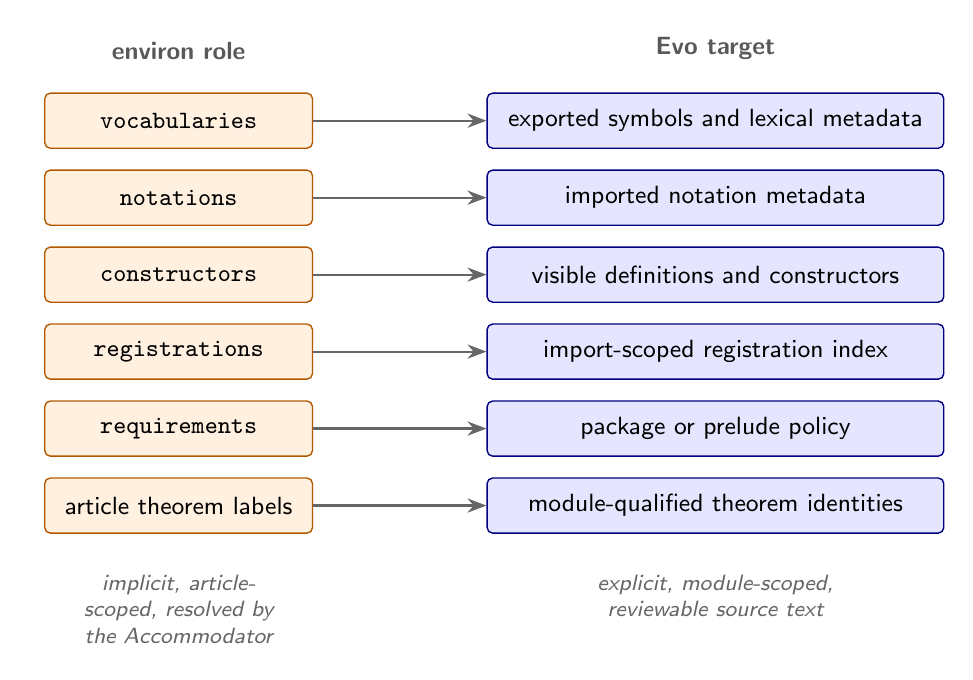
\begin{tikzpicture}[
  font=\sffamily,
  role/.style={draw, rounded corners=2pt, align=center, minimum width=34mm,
               minimum height=7mm, line width=0.5pt, fill=orange!12,
               draw=orange!70!black, font=\sffamily\small},
  target/.style={draw, rounded corners=2pt, align=center, minimum width=58mm,
                 minimum height=7mm, line width=0.5pt, fill=blue!10,
                 draw=blue!50!black, font=\sffamily\small},
  head/.style={font=\sffamily\small\bfseries, text=black!65},
  flow/.style={-{Stealth[length=2.4mm]}, line width=0.8pt, black!60},
  node distance=2.6mm,
]
  \node[role] (voc) {\texttt{vocabularies}};
  \node[role, below=of voc] (not) {\texttt{notations}};
  \node[role, below=of not] (con) {\texttt{constructors}};
  \node[role, below=of con] (reg) {\texttt{registrations}};
  \node[role, below=of reg] (req) {\texttt{requirements}};
  \node[role, below=of req] (thm) {article theorem labels};

  \node[target, right=22mm of voc] (tvoc) {exported symbols and lexical metadata};
  \node[target, right=22mm of not] (tnot) {imported notation metadata};
  \node[target, right=22mm of con] (tcon) {visible definitions and constructors};
  \node[target, right=22mm of reg] (treg) {import-scoped registration index};
  \node[target, right=22mm of req] (treq) {package or prelude policy};
  \node[target, right=22mm of thm] (tthm) {module-qualified theorem identities};

  \foreach \a/\b in {voc/tvoc, not/tnot, con/tcon, reg/treg, req/treq, thm/tthm}
    \draw[flow] (\a) -- (\b);

  \node[head, above=3mm of voc] {environ role\\[-2pt]};
  \node[head, above=3mm of tvoc] {Evo target\\[-2pt]};

  \node[font=\sffamily\footnotesize\itshape, text=black!60, below=4mm of thm,
        align=center, text width=36mm]
    {implicit, article-scoped, resolved by the Accommodator};
  \node[font=\sffamily\footnotesize\itshape, text=black!60, below=4mm of tthm,
        align=center, text width=56mm]
    {explicit, module-scoped, reviewable source text};
\end{tikzpicture}
\end{document}
